\chapter{Ideal cells, ordered gluing, and complete cusps}\label{ch:geometry}

\section{Why the local volume identity is not enough}
The angle identity \eqref{eq:gate-atoms} proves concavity, but an abstract sum of tetrahedral volumes is not yet the volume of a link complement. We construct the cells, identify the ordered input maps, and then compare the closed colored boundary with the literal projection cut. This supplies both the topology and the degree of the geometric realization. The construction does not require a polyhedron existence theorem; Rivin's variational approach \cite{Rivin1994} provides useful context, but is not a premise of this explicit argument.

\section{The leaf pyramid}
In upper half-space, place the apex at $O=\infty$ and the ordered port vertices at
\begin{equation}\label{eq:leaf-vertices}
 (C_0,C_1,C_2,C_3)=(1,e^{2\pi\ii a},-1,-e^{2\pi\ii a}),
 \qquad 0<a<1/2.
\end{equation}
Their convex hull is an ideal quadrangular pyramid. Its four apex edges are right angled. The base edge angles alternate $\pi a$ and $\pi(1/2-a)$. A diagonal of the base gives the two tetrahedra of \eqref{eq:leaf-atoms}, so its volume is $\pi g(a)$. Color the side triangles $(O,C_1,C_2)$ and $(O,C_3,C_0)$ shaded; the other two side triangles are white. The base is the output port.

Call edges $01,23$ of an output port \emph{free}, and edges $12,30$ \emph{cap}. A leaf has free angles $\pi a$ and cap angles $\pi(1/2-a)$. A completed cell will have free angles $\pi b$ and cap angles $\pi(1-b)$.

\begin{figure}[ht]
\centering
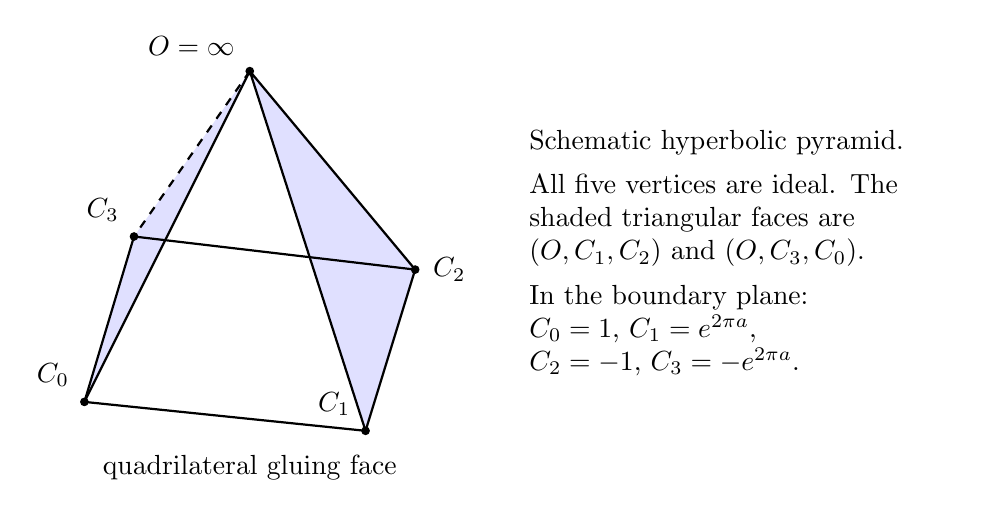
\begin{tikzpicture}[scale=1.05]
\coordinate (c0) at (-2,-1);\coordinate(c1) at (1.4,-1.35);\coordinate(c2) at (2,.6);\coordinate(c3) at (-1.4,1);\coordinate(o) at (0,3);
\fill[blue!12] (o)--(c1)--(c2)--cycle;\fill[blue!12] (o)--(c3)--(c0)--cycle;
\draw[thick] (c0)--(c1)--(c2)--(c3)--cycle;
\draw[thick] (o)--(c0) (o)--(c1) (o)--(c2);\draw[thick,dashed] (o)--(c3);
\foreach \p/\l in {c0/C_0,c1/C_1,c3/C_3,o/O=\infty}{\fill (\p) circle(1.5pt);\node[above left=2pt] at (\p) {$\l$};}
\fill (c2) circle(1.5pt);\node[right=3pt] at (c2) {$C_2$};
\node at (0,-1.8) {quadrilateral gluing face};
\node[align=left,text width=5.5cm] at (6,.8) {Schematic hyperbolic pyramid.\\[4pt]All five vertices are ideal. The shaded triangular faces are $(O,C_1,C_2)$ and $(O,C_3,C_0)$.\\[4pt]In the boundary plane:\\ $C_0=1$, $C_1=e^{2\pi\ii a}$,\\ $C_2=-1$, $C_3=-e^{2\pi\ii a}$.};
\end{tikzpicture}

\caption{One leaf contributes two shaded crossing-disk triangles and one ordered port. The one-leaf cap angle is $\pi(1/2-a)$; replacing it by the completed cap angle would give the wrong seam.}\label{fig:leaf}
\end{figure}

\section{The multiplication prism}
For a strict product define $p,q,r,w$ as in Chapter~\ref{ch:entropy}. In the boundary plane set
\begin{equation}\label{eq:prism-vertices}
 v_0=1,\quad v_1=e^{2\pi\ii p},\quad
 v_2=e^{2\pi\ii(p+r)},\quad
 v_3=e^{2\pi\ii(p+r+q)}.
\end{equation}
The consecutive half-arcs are $p,r,q,r+w$. Let $P$ be the intersection of the lines $(v_0,v_1)$ and $(v_2,v_3)$. The Euclidean triangle $(P,v_1,v_2)$ has positive angles $\pi y,\pi x,\pi w$, and the sine rule gives
\begin{equation}\label{eq:prism-P}
 P=v_1+\frac{\sin\pi x\sin\pi r}{\sin\pi w\sin\pi p}(v_1-v_0)
  =v_2+\frac{\sin\pi y\sin\pi r}{\sin\pi w\sin\pi q}(v_2-v_3).
\end{equation}
In particular $|P|>1$. Attach the tetrahedron $(\infty,P,v_1,v_2)$ to the quadrangular pyramid $(\infty,v_0,v_1,v_2,v_3)$, on opposite sides of their common face. The two coplanar face pairs merge. The result is a convex ideal triangular prism with white triangular faces $(P,v_1,v_2)$ and $(\infty,v_0,v_3)$ and ordered ports
\begin{equation}\label{eq:prism-ports}
 F_x=(\infty,v_0,v_1,P),\quad
 F_y=(\infty,v_3,v_2,P),\quad
 F_z=(v_0,v_1,v_2,v_3).
\end{equation}
\begin{figure}[ht]
\centering
\begin{tikzpicture}[scale=2.1, every node/.style={font=\small}]
\coordinate(v0) at (1,0);
\coordinate(v1) at ({cos(43.2)},{sin(43.2)});
\coordinate(v2) at ({cos(79.2)},{sin(79.2)});
\coordinate(v3) at ({cos(140.4)},{sin(140.4)});
\coordinate(P) at (0.57935,1.06242);
% Exact intersection of the two extended chords is used below.
\path[name path=first] (v0)--($(v0)!3!(v1)$);
\path[name path=second] (v3)--($(v3)!3!(v2)$);
\path[name intersections={of=first and second,by=P}];
\draw[gray] (0,0) circle(1);
\fill[blue!10] (P)--(v1)--(v2)--cycle;
\draw[thick] (v0)--(P)--(v3)--cycle;
\draw[thick] (v0)--(v1)--(v2)--(v3);
\draw[dashed] (v1)--(v3);
\foreach \p/\lab/\pos in {v0/v_0/right,v1/v_1/right,v2/v_2/left,v3/v_3/left,P/P/above}
 {\fill (\p) circle(.7pt);\node[\pos=2pt] at(\p){$\lab$};}
\node at (0,-1.3) {$p=.12,\quad r=.10,\quad q=.17,\quad w=.51$};
\node[align=left,text width=5.2cm] at (2.6,.3) {Boundary-plane construction.\\[3pt]$P=(v_0v_1)\cap(v_2v_3)$ lies outside the unit circle.\\[3pt]The sixth ideal vertex is $\infty$. The three quadrilateral gluing faces have ordered vertices $(\infty,v_0,v_1,P)$, $(\infty,v_3,v_2,P)$ and $(v_0,v_1,v_2,v_3)$.};
\end{tikzpicture}

\caption{The exact boundary-plane construction of a strict prism at one rational angle tuple. The lines and circle are the defining support data; the drawing is not a perspective view of the three-dimensional hyperbolic cell.}\label{fig:prism}
\end{figure}

Its edge angles, divided by $\pi$, are
\begin{center}
\begin{tabular}{ll}\toprule
Edges & Angle\\\midrule
$Pv_1,\ \infty v_0$ & $x$\\
$Pv_2,\ \infty v_3$ & $y$\\
$v_1v_2,\ v_0v_3$ & $1-z$\\
$P\infty$ & $w$\\
$v_0v_1$ & $p$\\
$v_2v_3$ & $q$\\\bottomrule
\end{tabular}
\end{center}
The support half-spaces are the three vertical planes over the lines through $P$ and over $(v_3,v_0)$, and the hemispheres through the two remaining face circles. Formula~\eqref{eq:prism-P} places the two attached pieces on the required sides. Equivalently, their seam is locally convex because its boundary angle sums are at most $\pi$. The volume is $\pi m(x,y,z)$: triangulate the pyramid across $v_0v_2$ and cancel the complementary intermediate Lobachevsky terms; the attached tetrahedron supplies $V(y,x,w)$.

\section{Stationarity matches whole ordered faces}
For cyclically ordered points on a circle or line, define
\[
 \varkappa(a,b,c,d)=\frac{(a-b)(c-d)}{(a-d)(b-c)}>0.
\]
Three ordered vertices can be sent to $(\infty,0,1)$, so this number determines the ordered ideal quadrilateral. A cyclic shift or the relevant reversal replaces it by its reciprocal. Direct substitution gives
\begin{align}
 \varkappa(F_x)&=\frac{\sin\pi x\sin\pi r}{\sin\pi w\sin\pi p},&
 \varkappa(F_y)&=\frac{\sin\pi y\sin\pi r}{\sin\pi w\sin\pi q},\notag\\
 \varkappa(F_z)&=\frac{\sin\pi p\sin\pi q}{\sin\pi z\sin\pi r}.\label{eq:face-metrics}
\end{align}
These are $e^{-m_x}$, $e^{-m_y}$ and $e^{-m_z}$, respectively. The leaf metric is $\tan^2\pi a=e^{-g'(a)}$.

The lower and upper stack maps are exactly
\begin{equation}\label{eq:ordered-stack}
 (C_0,C_1,C_2,C_3)\mapsto(v_0,v_1,P,\infty),\qquad
 (C_0,C_1,C_2,C_3)\mapsto(\infty,P,v_2,v_3).
\end{equation}
Both invert the port metric. At each internal wire, stationarity says that the child output derivative and parent input derivative sum to zero. Hence $\varkappa_{\rm child}\varkappa_{\rm parent}=1$, precisely the isometry condition for \eqref{eq:ordered-stack}. This verifies the full face map, rather than only an edge-product equation.

\section{Convex assembly and the closed cut}
Attach child cells to the two prism inputs on opposite supported sides. A leaf cap edge meets a prism edge with total angle $\pi/2$; a completed cap edge gives $\pi$ and merges two white faces. The common input edge has angle $\pi(w+x+y)=\pi$. The two free output seams have angles $\pi(p+x)=\pi z$ and $\pi(q+y)=\pi z$, while the cap output angles are $\pi(1-z)$.

These inequalities prove local convexity at each finite seam. To justify global convexity directly, a length-minimizing sequence between two finite points of the union stays in a compact hyperbolic ball. A shortest path exists. Local convexity makes it an ambient geodesic at every finite point, so it is the unique ambient segment and lies in the union. Ideal vertices are not finite points and introduce no additional exception. Thus each completed expression gives a convex ideal cell with one supported port and the claimed free/cap pattern. Its nonport edges remain right angled, and its two shaded triangles per leaf keep their labels.

At the final closure, the outputs are $b$ and $1-b$. Stationarity gives equal ordered port metrics. The gluing is
\begin{equation}\label{eq:closing-map}
 F:C_j\longmapsto G:C_{3-j}\qquad(j\bmod4).
\end{equation}
It implements both the stack interface and the two outside closing wires. Free and cap angles each sum to $\pi$ for two completed children. After merging flat white seams, the result is a convex right-angled ideal polyhedron $P_E$. It has $2H$ shaded triangles, $H+2$ white faces, $3H$ ideal vertices and $6H$ edges. These counts are checks, not the proof of topology.

For topology, cut the literal augmented diagram along its projection sphere and the recorded half crossing disks. In each projection ball the auxiliary semicircles are boundary-parallel along those half disks. Drilling them and then cutting returns a ball. A disk contributes precisely the two shaded triangles $(O,C_1,C_2)$ and $(O,C_3,C_0)$. The remaining regions are white. The original stack identifies lower corners $2,3$ with upper corners $1,0$ and preserves the exposed order $(F_0,F_1,G_2,G_3)$. Turns rotate that order, and the final closure pairs $0$ with $3$ and $1$ with $2$. These rules determine every oriented white facial walk. They are exactly the rules induced by \eqref{eq:ordered-stack} and \eqref{eq:closing-map}. The labeled sphere cellulation therefore agrees with the projection cut; its identification extends over each ball. Reversing the cuts gives the stated link exterior with degree one.

\section{Complete cusps and half-twist partners}
Take two oppositely oriented copies of $P_E$. Pair white faces between copies by their projection labels. In a pure leaf, pair its two shaded triangles within each copy, fixing $O$ and sending $C_1\mapsto C_0$, $C_2\mapsto C_3$. The edge words alternate white and shaded gluings, contain four right angles, and return pointwise: the copied white maps and the inverse triangle maps cancel. Thus there is no translation along an edge hidden by an angle count.

At each ideal vertex, a horosphere cuts a Euclidean rectangle. Scale it so that its two opposite shaded sides have length one. Every shaded triangle then has the same canonical corner horocycles. All shaded and white pairings preserve the decoration. Uniform shrinking makes the horospheres disjoint. The links glue without dilation to the actual compact cusp tori, while their complement is compact. The resulting metric is complete and has volume
\begin{equation}\label{eq:complete-volume}
 \Vol(Y_E^0)=2\Vol(P_E)=2\pi F_0.
\end{equation}

A half twist rotates one side of the twice-punctured disk by $\pi$, exchanging both punctures and the upper/lower half disks. Hence the shaded maps become
\[
 S_0^+\to S_1^-:\ (O,C_1,C_2)\mapsto(O,C_3,C_0),\qquad
 S_1^+\to S_0^-:\ (O,C_3,C_0)\mapsto(O,C_1,C_2).
\]
They go across the two copies, not within one copy. White maps are unchanged. The explicit edge matrices in Chapter~\ref{ch:marked} show pointwise cancellation of all three odd edge words. The length-one triangle decorations are also preserved, so every fixed half-twist pattern has the same complete volume $2\pi F_0$. The two half-twist signs have the same unmarked pairing but different collar paths; those paths are kept for filling.

\section{A constructive knot choice}\label{sec:pairings}
For ports $(0,1,2,3)$ in cyclic order, write
\[
 I=(0,3)(1,2),\qquad U=(0,1)(2,3),\qquad X=(0,2)(1,3).
\]
A pure leaf gives $U$ and an odd leaf gives $X$. Turn exchanges $I,U$ and fixes $X$. Tracing the two stack wires gives
\begin{center}
\begin{tabular}{c|ccc}
 lower/upper & $I$ & $U$ & $X$\\\hline
$I$ & $I$ & $U$ & $X$\\
$U$ & $U$ & $U$ plus an internal circle & $U$\\
$X$ & $X$ & $U$ & $I$
\end{tabular}
\end{center}
Only $U\cdot U$ creates an internal component. The base $hh$ offers $\{I,U\}$ without such a component. Every product of two feasible two-element subsets of $\{I,U,X\}$, after deleting the forbidden choice, still offers at least two elements; the same holds when one child is the leaf set $\{U,X\}$. Turn permutes the choices. Induction gives at least two loop-free choices for every completed expression. At the root choose $U$ or $X$, whose cylindrical closure is one component, and backtrack the finite choices. Either sign realizes an odd leaf. Full twists have even endpoint permutation, so all subsequent auxiliary fillings preserve the one main component.
